\section{Auswertung}
\label{sec:Auswertung}

Zunächst wird der Acrylblock mit einer Schieblehre vermessen.
Die Messwerte für die einzelnen Löcher sind in Tabelle \ref{tab:schieblehre} dargestellt.
Die Nummern der Bohrungen können der Abbildung \ref{fig:kenblock} entnommen werden.
Die Abmessungen des Blockes lauten:

\begin{align*}
  \text{Breite} &= \SI{150.25}{\milli\metre} \\
  \text{Höhe}   &= \SI{80.45}{\milli\metre} \\
  \text{Tiefe}  &= \SI{40.00}{\milli\metre}
\end{align*}

Wichtig ist für die folgenden Veruchsteile lediglich die Höhe des Blockes.

\begin{table}
  \centering
  \caption{Abmessungen der Bohrungen innerhalb des Acrylblockes.}
  \label{tab:schieblehre}
  \begin{tabular}[t]{c c c c}
   \toprule
    {Nummer} & {$l_\text{oben}$ / $\si{\milli\metre}$} & {$l_\text{unten}$ / $\si{\milli\metre}$} &  {Dicke / $\si{\milli\metre}$} \\
     \midrule
     \csvreader[no head,
     late after line=\\,
     late after last line=\\\bottomrule]%
     {data/abmessungentab.csv}{}%
     {$\num{\csvcoli}$ & $\num{\csvcolii}$ & $\num{\csvcoliii}$ & $\num{\csvcoliv}$ }%
   \end{tabular}
 \end{table}

\FloatBarrier
\subsection{Untersuchung eines Acrylblockes mit dem A-Scan}

Die Laufzeit der Schallwellen durch den Acrylblock bis zu der Störstelle ist in Tabelle \ref{tab:ascan} dargestellt.
Für die Umrechnung der Zeiten in die Länge wird Gleichung \eqref{eqn:wegzeit} genutzt.
Die Schallgeschwindigkeit in Acryl beträgt dabei $\SI{2730}{\metre\per\second}$ \cite{acryl}.
Da die Sonde nicht unmittelbar auf dem Acrylblock ruht, sondern auf einem Film aus bidestilliertem Wasser muss aus jeder Rechnung die Zeit herausgerechnet werden, die der Ultraschall benötigt um das Koppelmittel zu durchqueren.
Dieser wurde zu $\SI{0.43}{\micro\second}$ bestimmt.
Für die Bestimmung der Dicke der Bohrungen wird erneut die Dicke des Acrylblockes benötigt.
Die Gesamtzeit, die der Ultraschall benötigt um den Block zu durchqueren beträgt $\SI{60.55}{\micro\second}$, bzw. $\SI{60.12}{\micro\second}$ unter Berücksichtigung des Kopplungsmittels.
Damit lässt sich die Höhe des Blockes auf $\SI{82.06}{\milli\metre}$ berechnen.

\begin{table}
  \centering
  \caption{Abmessungen der Bohrungen innerhalb des Acrylblockes.}
  \label{tab:ascan}
  \begin{tabular}[t]{c c c c c c}
   \toprule
    {Nummer} & {$t_\text{oben}$ / $\si{\micro\second}$} & {$l_\text{oben}$ / $\si{\milli\metre}$} & {$t_\text{unten}$ / $\si{\micro\second}$} & {$l_\text{unten}$ / $\si{\milli\metre}$} &  {Dicke / $\si{\milli\metre}$} \\
     \midrule
     \csvreader[no head,
     late after line=\\,
     late after last line=\\\bottomrule]%
     {data/ascantab.csv}{}%
     {$\num{\csvcoli}$ & $\num{\csvcolii}$ & $\num{\csvcoliii}$ & $\num{\csvcoliv}$ & $\num{\csvcolv}$ & $\num{\csvcolvi}$ }%
   \end{tabular}
 \end{table}

Das Auflösungsvermögen der $\SI{2}{\mega\hertz}$-Sonde wird in Tabelle \ref{tab:auflösung} dargestellt.
Die entsprechenden Daten für die Löcher 1 und 2 der $\SI{1}{\mega\hertz}$-Sonde befinden sich in Tabelle \ref{tab:ascan}.

\begin{table}
  \centering
  \caption{Daten zum Auflösungsvermögen der $\SI{2}{\mega\hertz}$-Sonde.}
  \label{tab:auflösung}
  \begin{tabular}[t]{c c c c c c}
   \toprule
    {Nummer} & {$t_\text{oben}$ / $\si{\micro\second}$} & {$l_\text{oben}$ / $\si{\milli\metre}$} & {$t_\text{unten}$ / $\si{\micro\second}$} & {$l_\text{unten}$ / $\si{\milli\metre}$} &  {Dicke / $\si{\milli\metre}$} \\
     \midrule
     \csvreader[no head,
     late after line=\\,
     late after last line=\\\bottomrule]%
     {data/auflosungtab.csv}{}%
     {$\num{\csvcoli}$ & $\num{\csvcolii}$ & $\num{\csvcoliii}$ & $\num{\csvcoliv}$ & $\num{\csvcolv}$ & $\num{\csvcolvi}$ }%
   \end{tabular}
 \end{table}

\subsection{Untersuchung eines Acrylblockes mit dem B-Scan}

Für den B-Scan wird eine $\SI{2}{\mega\hertz}$-Sonde verwendet.
Die aufgezeichneten Bilder sind in Abbildung \ref{fig:Boben} und \ref{fig:Bunten} dargestellt.
Aus diesen Bildern werden erneut die Abmessungen der Störstellen berechnet.
Die abgelesenen und berechneten Daten sind in Tabelle \ref{tab:bscan} zu finden.
Die Berechnung der Länge in Millimetern und der Dicke erfolgt analog zum A-Scan.
Die Daten von Loch 10 konnten für die Messung der Unterseite nicht hinreichend aufgeklöst werden.
Dieser Wert entfällt daher.
Auch hier muss erneut die Koppelschicht berücksichtigt werden.
Der Ultraschall benötigt  $\SI{2.58}{\micro\second}$ zum Durchqueren.
Dies wird aus den Werten herausgerechnet.
Die Höhe des Blockes wurde für beide Scans zu $\SI{56.23}{\micro\second}$, bzw. $\SI{76.75}{\milli\metre}$ berechnet.

\begin{figure}
  \centering
  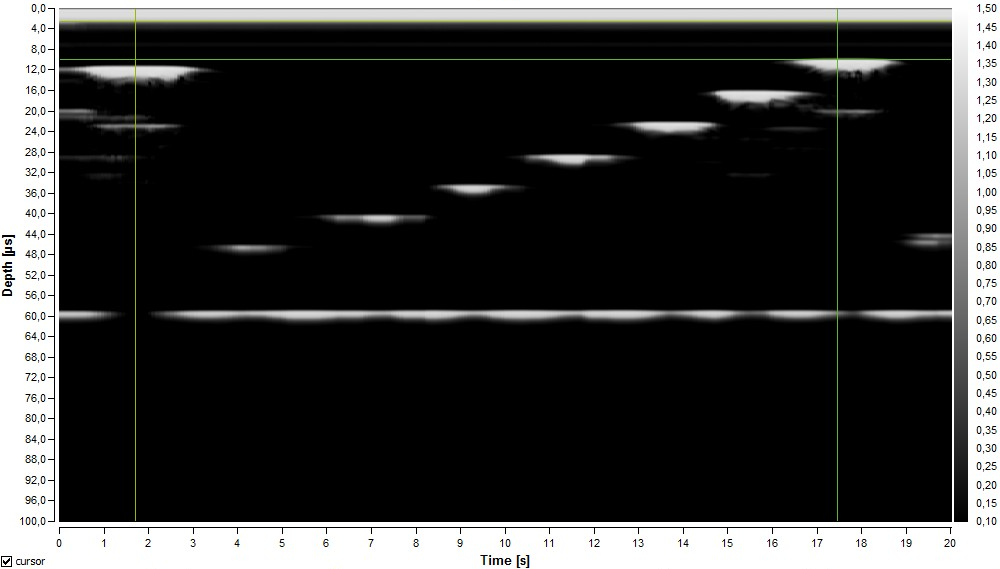
\includegraphics[width=0.7\textwidth]{images/bscanoben.png}
  \caption{Aufzeichnung des B-Scans für die Oberseite des Acrylblockes.}
  \label{fig:Boben}
\end{figure}

\begin{figure}
  \centering
  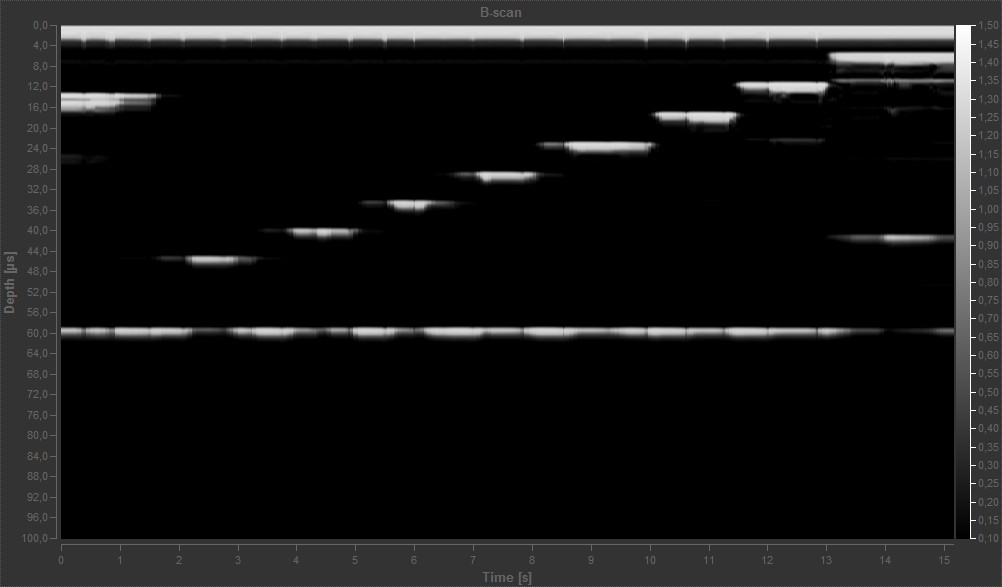
\includegraphics[width=0.7\textwidth]{images/bscanunten.png}
  \caption{Aufzeichnung des B-Scans für die Unterseite des Acrylblockes.}
  \label{fig:Bunten}
\end{figure}

\begin{table}
  \centering
  \caption{Die Messergebnisse für die Vermessung des Acrylblockes mithilfe des B-Scans.}
  \label{tab:bscan}
  \begin{tabular}[t]{c c c c c c}
   \toprule
    {Nummer} & {$t_\text{oben}$ / $\si{\micro\second}$} & {$l_\text{oben}$ / $\si{\milli\metre}$} & {$t_\text{unten}$ / $\si{\micro\second}$} & {$l_\text{unten}$ / $\si{\milli\metre}$} &  {Dicke / $\si{\milli\metre}$} \\
     \midrule
     \csvreader[no head,
     late after line=\\,
     late after last line=\\\bottomrule]%
     {data/bscantab.csv}{}%
     {$\num{\csvcoli}$ & $\num{\csvcolii}$ & $\num{\csvcoliii}$ & $\num{\csvcoliv}$ & $\num{\csvcolv}$ & $\num{\csvcolvi}$ }%
   \end{tabular}
 \end{table}

\begin{figure}
  \centering
  \includegraphics{plot.pdf}
  \caption{Plot.}
  \label{fig:plot}
\end{figure}
